\documentclass[10pt]{article}
%----------Packages----------
\usepackage[utf8]{inputenc}
\usepackage[landscape,left=5mm,right=5mm,top=5mm,bottom=5mm]{geometry}
\usepackage{amsmath,amssymb}
\usepackage{siunitx}
\usepackage{multicol}
\usepackage{blindtext}
\usepackage{graphicx}
\usepackage{bm}
\usepackage{tikz}
\usetikzlibrary{angles, quotes, calc}

%----------Page formatting----------
\pagenumbering{gobble}
\setlength{\parindent}{0pt}

%----------Symbols----------
\newcommand{\ep}{\varepsilon}
\newcommand{\al}{\alpha}
\renewcommand{\th}{\theta}
\newcommand{\om}{\omega}

%----------General----------
\newcommand{\ds}{\displaystyle}
\newcommand{\tab}{\hspace{.02\textwidth}}
\newcommand{\twoEqn}[4]{$\makebox[#3][l]{$#1$} \makebox[#4][l]{$#2$}$}
\newcommand{\threeEqn}[6]{$\makebox[#4][l]{$#1$} \makebox[#5][l]{$#2$} \makebox[#6][l]{$#3$}$}
\newcommand{\splittab}{\hspace{2.58ex}}

%----------Math----------
\renewcommand{\d}{\,d}
\newcommand{\p}{\partial}
\newcommand{\dv}[2]{\frac{\mathrm{d} #1}{\mathrm{d} #2}}
\newcommand{\ddv}[2]{\frac{\mathrm{d}^2 #1}{\mathrm{d} #2^2}}
\newcommand{\pd}[2]{\frac{\partial #1}{\partial #2}}
\newcommand{\pdd}[2]{\frac{\partial^2 #1}{\partial #2^2}}
\newcommand{\inv}{^{-1}}

%----------Brackets----------
\newcommand{\lrb}[1]{\left(#1\right)}
\newcommand{\sqb}[1]{\left[#1\right]}
\newcommand{\abs}[1]{\left|#1\right|}
\let\originalleft\left
\let\originalright\right
\renewcommand{\left}{\mathopen{}\mathclose\bgroup\originalleft}
\renewcommand{\right}{\aftergroup\egroup\originalright}

%----------Sections----------
\makeatletter
\renewcommand{\section}{\@startsection{section}{1}{0ex}{-1ex}{0.7ex}
                        {\normalfont\large\bfseries}}
\renewcommand{\subsection}{\@startsection{subsection}{2}{0ex}{-0.4ex}{0.4ex}
                        {\normalfont\normalsize\bfseries}}
\makeatother
\setcounter{secnumdepth}{0}

%----------ENPH 270----------
\newcommand{\cross}{\times}
\newcommand{\bs}{\boldsymbol}
\newcommand{\bv}[1]{\mathbf{#1}}
\newcommand{\uv}[1]{{\bm{\hat{\textnormal{\bfseries #1}}}}}
\renewcommand{\r}{\bv r}
\renewcommand{\v}{\bv v}
\renewcommand{\a}{\bv a}
\newcommand{\ih}{\uv{\i}}
\newcommand{\jh}{\uv{\j}}
\newcommand{\kh}{\uv{k}}
\newcommand{\Rel}{\text{Rel}}
\newcommand{\A}{\bv A}
\newcommand{\B}{\bv B}
\newcommand{\C}{\bv C}

\usepackage[mathscr]{eucal}

%----------Document Begins Here----------
\begin{document}

\begin{multicols*}{3}
\raggedcolumns

{\LARGE{\underline{ENPH 270 Formula Sheet}}}

\section{Basics}

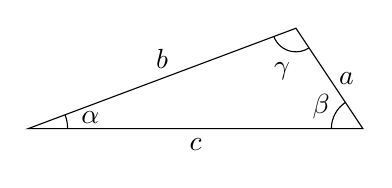
\begin{tikzpicture}[scale=0.85]
    \coordinate (A) at (0,0);
    \coordinate (B) at (5,0);
    \coordinate (C) at (4,1.5);
    \draw (A) -- (B) -- (C) -- cycle;

    \coordinate[label=below:$c$](c) at ($ (A)!.5!(B) $);
    \coordinate[label=right:$a$](a) at ($ (B)!.5!(C) $);
    \coordinate[label=above:$b$](b) at ($ (C)!.5!(A) $);

    \pic[draw, angle eccentricity=1.6, angle radius=5mm, "$\alpha$"] {angle = B--A--C};
    \pic[draw, angle eccentricity=1.5, angle radius=4mm, "$\beta$"] {angle = C--B--A};
    \pic[draw, angle eccentricity=1.9, angle radius=3mm, "$\gamma$"] {angle = A--C--B};
\end{tikzpicture}

Sine Law:

\tab $\frac{a}{\sin\alpha}=\frac{b}{\sin\beta}=\frac{c}{\sin\gamma}$

Cosine Law:

\tab $a^2=b^2+c^2-2bc\cos\alpha$

Cross Product:

\tab \threeEqn{\ih\cross\jh=\kh}{\jh\cross\kh=\ih}{\kh\cross\ih=\jh}{7em}{7em}{7em}

\tab \threeEqn{\ih\cross\kh=-\jh}{\jh\cross\ih=-\kh}{\kh\cross\jh=-\ih}{7em}{7em}{7em}

BAC-CAB Rule:

\tab $\A\times\B\times\C=\B(\A\cdot\C)-\C(\A\cdot\B)$

\section{Planar Kinematics}

Constant Acceleration:

\tab \twoEqn{v(t)=v_0+at}{\om(t)=\om_0+\al t}{12em}{11em}

\tab \twoEqn{x(t)=x_0+v_0t+\frac{1}{2}at^2}{\th(t)=\th_0+\om_0+\frac{1}{2}\al t^2}{12em}{11em}

\tab \twoEqn{v^2=v_0^2+2a(x-x_0)}{\om^2=\om_0^2+2\al(\th-\th_0)}{12em}{11em}

Velocity and Acceleration:

\tab \twoEqn{v\d v=a\d x}{\om\d\om=\al\d\th}{12em}{11em}

General Planar Motion:

\tab $\r_B=\r_A+\r_{B/A}$

\tab $\v_B=\v_A+\bs\omega\cross\r_{B/A}$

\tab $\a_B=\a_A+\bs\alpha\cross\r_{B/A}-\omega^2\r_{B/A}$

Instantaneous Center of Rotation (ICR):

\tab $\v_A=\bs\omega\cross\r_{A/O}$

Rotating Axes:

\tab $\v_B=\v_A+\bs\omega\cross\r_{B/A}+\lrb{\v_B}_\Rel$

\tab $\a_B=\a_A+\bs\alpha\cross\r_{B/A}-\omega^2\r_{B/A}+\lrb{\a_B}_\Rel+2\bs\omega\times\lrb{\v_B}_\Rel$

\section{Planar Kinetics: Force and Acceleration}

Center of Mass:

\tab $(x_G,y_G)=\lrb{\frac 1M\sum_{i}m_ix_i, \frac 1M\sum_{i}m_iy_i}$

Moment of Inertia:

\tab $I=\int_m r^2\d m$

Parallel Axis Theorem:

\tab $I_A=I_G+md^2$

Radius of Gyration:

\tab $I=mk^2$

Planar Equations of Motion:

\tab $\sum F_x=m(a_G)_x$

\tab $\sum F_y=m(a_G)_y$

\tab $\sum M_G=I_G\alpha$

\tab $\sum M_A=I_G\alpha+\abs{\r_{G/A}\cross(m\a_G)}$

\tab $\sum M_A=I_A\alpha+\abs{\r_{G/A}\cross(m\a_A)}$

Rectilinear Translation:

\tab $\sum M_G=0$

\tab $\sum M_A=(ma_G)d$

Curvilinear Translation:

\tab $\sum F_n=m(a_G)_n=m\omega^2 r_G$

\tab $\sum F_t=m(a_G)_t=m\alpha r_G$

\section{Planar Kinetics: Work and Energy}

Kinetic Energy:

\tab $T=\frac 12mv_G^2+\frac 12I_G\omega^2$

\tab $T=\frac 12I_O\omega^2$

Potential Energy:

\tab $V_g=mgy_G$

\tab $V_e=\frac 12ks^2$

Work:

\tab $U=\int_s F\cos\theta\d s$

\tab $U_W=-W\Delta y$

\tab $U_S=-\lrb{\frac 12ks_2^2-\frac 12ks_1^2}\qquad \abs{s_2}>\abs{s_1}$

Principle of Work and Energy:

\tab $T_1+U_{1\rightarrow 2}=T_2$

\tab $T_1+V_1+U_{1\rightarrow 2}^{\text{(non-cons)}}=T_2+V_2$

\rule{\linewidth}{0.1pt}

{\scriptsize 
Compiled \today}

\end{multicols*}

\end{document}